%-----------------------------------------------
% Dateiname: IntegrationInstallTool.tex
% Autor    : Stefano Kowalke <blueduck@gmx.net>
% Lizenz   : BSD
%-----------------------------------------------
\section{Integration des Prototypen in das Install Tool}
\label{prototype:sec:integrateIntoInstallTool}
Um bereits bei der Installation ein alternatives \gls{dbms} nutzen zu können, mußte der Prototyp bereits über das \textit{Install Tool} installierbar sein, was Anpassungen an dem \textit{Install Tool} und TYPO3 CMS zur Folge hatte.

Wie in Kapitel~\ref{prototype:subsec:installTYPO3} zu sehen war, besteht das \textit{Install Tool} aus fünf Schritten, die durch die Klassen im Ordner \pdf{typo3/sysext/install/Classes/Controller/Action/Step} bereitgestellt werden. Der \phpinline{\TYPO3\CMS\Install\Controller\StepController} iteriert bei jedem Reload des Installtools über alle Schritte und prüft ob der jeweils aktuelle Schritt bereits ausgeführt wurde oder noch ausgeführt werden muß. Er erkennt dies an Bedingungen, die von jedem Schritt definiert werden. Sind alle Bedingungen erfüllt, findet ein Redirekt auf den nächsten Schritt statt.

Die Ausgabe der Schritte erfolgt über verschiedene HTML-Template Dateien, die in der TYPO3 eigenen Template-Sprache \textit{Fluid} verfasst sind. Das \textit{Install Tool} setzt hier das \gls{mvc}-Pattern ein, um die Geschäftslogik von der Präsentation zu trennen.

Die HTML-Templates unterteilen sich in \textit{Layouts}, \textit{Templates} und \textit{Partials}, die in den jeweilig gleichnamigen Verzeichnissen in \pdf{typo3/sysext/install/Resources/Privat/} zu finden sind.

\begin{itemize}
	\item Ein Template beschreibt die grundlegende Struktur einer Seite. Typischerweise befindet sich darin der Seitenkopf und -fuß.
	\item Die Struktur einer einzelnen Seite wird von einem Template festgelegt.
	\item Partials stellen wiederkehrende Elemente dar. Sie können in Layout- und Templatedateien eingebunden werden. Die Schaltfläche \textit{I do not use MySQL} aus Abbildung~\ref{fig:installTYPO3LegacyStepTwo} in Kapitel~\ref{prototype:subsec:TwoInsertDatabaseData} ist ein Beispiel für ein Partials.
\end{itemize}


Im Folgenden werden die vorgenommenen Änderungen im Detail beschrieben.

\begin{itemize}
\item In \phpinline{\TYPO3\CMS\Core\Core\Bootstrap} wurde die von Composer erstellte\\ \textit{Autoload}-Datei eingebunden. Somit können die von Doctrine DBAL zur Verfügung gestellten Klassen geladen werden. Siehe Listing~\ref{lst:composerAutoload}
\item Es wurden die Partials \pdf{LoadDoctrineDbal.html} und \pdf{UnloadDoctrineDbal.html} zur De- und Installation des Prototypen sowie das Partial\\ \pdf{DoctrineDbalDriverSelection.html} für die Auswahl des Datenbanktreibers erstellt und wurden dem Template des zweiten Schritts \pdf{DatabaseConnect.html} hinzugefügt. Die Variable \texttt{isDoctrineEnabled} enthält den Installationsstatus des Prototypen. Abhängig von ihr wird entweder die Schaltfläche zur Installation des Prototypen oder das Auswahlfeld für die Datenbanktreiber und die Schaltfläche zur Deinstallation des Prototypen anzeigt.
\item Damit die Variable einen Wert enthält, wurde diese von der \textit{Action} aus\\ \phpinline{\TYPO3\CMS\Install\Controller\Action\Step\DatabaseConnect} definiert und an die View übergeben.
\item in \phpinline{\TYPO3\CMS\Install\Controller\Action\Step\DatabaseConnect} wurden Methoden erstellt, die die installierten PDO-Extensions des Systems abfragen und an die View übergeben
\item Zur Vermeidung leerer Werte in der Konfigurationsdatei, wurden die Prüfungen der Benutzereingaben von \phpinline{isset()} auf \phpinline{!empty()} geändert.
\item Das Eingabeformular für die Datenbankverbindungsinformationen wurde angepasst. Es wurde ein Feld für das \textit{Charset} der Datenbank hinzugefügt und das Feld für die Datenbank entfernt, da sie in einem anderen Schritt über ein Auswahlfeld festgelegt wird.
\item Damit die eingegebenen Daten weiterverarbeitet werden konnten, wurden diese in den entsprechenden PHP-Klassen ergänzt.
\item Externe Abhängigkeiten werden vom Package Manager in\\ \pdf{thesis.dev/http/Packages/Library} erwartet. Aus diesem Grund mußte der Ordner \pdf{doctrine\_dbal/vendor/doctrine} nach \pdf{thesis.dev/http/Packages/Library/} kopiert werden.\footnote{Composer Konfigurationsdateien werden seit TYPO3 CMS 6.2 analysiert. Aus den definierten Abhängigkeiten und den (System)-Extensions wird vom Package Mananger ein Graph von Abhängigkeiten aufgebaut welcher in \pdf{thesis.dev/http/typo3conf/PackagesStates.php} gespeichert wird. Diese Datei wird bei der Installation erstellt und stetig aktualisiert. Da diese Funktionalität relativ neu ist, mußte diese Datei bei der Installation des Prototypen manuell angepasst werden.}
\end{itemize}

\begin{listing}[H]
\begin{phpcode}
// Bootloader.php
public function initializeClassLoader() {
	/** Composer loader */
	require_once PATH_typo3conf . 'ext/doctrine_dbal/vendor/autoload.php';

	$classLoader = new ClassLoader($this->applicationContext);
	...
}
\end{phpcode}
\caption{Einbinden des vom Composer erstellten Autoloaders}
\label{lst:composerAutoload}
\end{listing}

%\begin{htmlcode}
%<f:if condition="{isDoctrineEnabled}">
	%<f:then>
		%<f:render partial="Action/Step/DatabaseConnect/DoctrineDbalDriverSelection" arguments="{_all}" />
		%<f:if condition="{selectedDoctrineDriver}">
			%<f:render partial="Action/Step/DatabaseConnect/ConnectDetails" arguments="{_all}" />
		%</f:if>
		%<f:render partial="Action/Step/DatabaseConnect/UnloadDoctrineDbal" arguments="{_all}" />
	%</f:then>

	%<f:else>
		%<f:render partial="Action/Step/DatabaseConnect/ConnectDetails" arguments="{_all}" />
		%<f:render partial="Action/Step/DatabaseConnect/LoadDoctrineDbal" arguments="{_all}" />
		%<f:render partial="Action/Step/DatabaseConnect/LoadDbal" arguments="{_all}" />
	%</f:else>
%</f:if>
%\end{htmlcode}

%\begin{listing}
%\begin{phpcode}
%$isDbalEnabled =
  %\TYPO3\CMS\Core\Utility\ExtensionManagementUtility::isLoaded('doctrine_dbal');

%$this->view
  %->assign('isDoctrineEnabled', $isDoctrineEnabled)
  %->assign('username', $this->getConfiguredUsername())
  %->assign('password', $this->getConfiguredPassword())
  %->assign('host', $this->getConfiguredHost())
  %->assign('port', $this->getConfiguredOrDefaultPort())
  %->assign('database', $GLOBALS['TYPO3_CONF_VARS']['DB']['database'] ?: '')
  %->assign('socket', $GLOBALS['TYPO3_CONF_VARS']['DB']['socket'] ?: '');
%\end{phpcode}
%\caption{Zuweisung von in PHP definierten Variablen an die View}
%\end{listing}

\subsection{Doctrines Schemarepr\"asentation}
\label{subsec:doctrineSchema}

Während der Installation werden die initialen Datenbanktabellen angelegt. Die dafür notwendigen \gls{sql}-Abfragen halten die Extensions in \pdf{*.sql}-Dateien vor. Dabei handelt es sich um einfache Textdateien, die aus ein oder mehreren \mysqlinline{CREATE TABLE} Abfragen bestehen.
Diese werden von \phpinline{TYPO3\CMS\Core\Database\SqlParser} geparst, auseinandergenommen und neu zusammengesetzt, wobei kleinere Syntaxfehler behoben werden. Eine Hauptaufgabe des Parsers liegt darin, diejenigen \pdf{*.sql}-Dateien zu erkennen und zu vereinen, die die gleiche Tabelle mit unterschiedlichen Feldern anlegen wollen. Als Beispiel seien die Systemextensions \texttt{ext:frontend} und \texttt{ext:felogin} erwähnt, die beide die Tabelle \texttt{fe\_users} anlegen.

\begin{listing}
\begin{mysqlcode}
# ext:felogin
CREATE TABLE fe_users (
	felogin_redirectPid  tinytext,
	felogin_forgotHash  varchar(80) default ''
);

# ext:frontend
CREATE TABLE fe_users (
	uid int(11) unsigned NOT NULL auto_increment,
	pid int(11) unsigned DEFAULT '0' NOT NULL,
	tstamp int(11) unsigned DEFAULT '0' NOT NULL,
	username varchar(50) DEFAULT '' NOT NULL,
	password varchar(100) DEFAULT '' NOT NULL,
	usergroup tinytext,
	…
);
\end{mysqlcode}
\caption{}
\label{lst:sameSQLDefinitionOfFeUsers}
\end{listing}

Der Importvorgang erfolgt durch die Methode \phpinline{importDatabaseData()} aus der Klasse \phpinline{\TYPO3\CMS\Install\Controller\Action\Step\DatabaseData}. Dabei ermittelt die Methode \phpinline{\TYPO3\CMS\Install\Service\SqlExpectedSchemaService::getTablesDefinitionString()} anhand der \pdf{*.sql}-Dateien den Soll-Zustand. Die Methode \phpinline{getFieldDefinitions_database()} aus der Klasse \phpinline{\TYPO3\CMS\Install\Service\SqlSchemaMigrationService} ermittelt den Ist-Zustand. Beide Zustände werden anschließend durch die Methoden \phpinline{getDatabaseExtra()} und \phpinline{getUpdateSuggestions()} derselben Klasse verglichen. Die genauere Analyse der Methoden würde für die Arbeit zu weit führen, deswegen wird hier darauf verzichtet. Anschließend wird die Differenz in Form von \gls{sql}-Abfragen an die Datenbank gesendet.


Statische Daten werden über Dateien mit der Bezeichnung \pdf{ext\_tables\_static+adt.sql} in die Datenbank eingefügt. Im Moment besitzt lediglich der Extension Manager solch eine Datei, die die URL zum \gls{ter} einfügt.

Um die Abhängigkeit des \textit{Install Tool} zu MySQL bei der Erstellung der Basistabellen aufzulösen, wurden die \pdf{*.sql}-Dateien in die Schema Syntax von Doctrine überführt. Dies wurde bereits in Kapitel~\ref{basics:doctrine:subsec:dbal} durch die Erstellung eines Schemas skizziert. Die Zielstellung war die vollständige Umstellung auf \phpinline{\Doctrine\DBAL\Schema\Schema}-Objekte, da diese die notwendige Abstraktion bieten und von Doctrine DBAL anhand der  verwendeten Plattform in die entsprechenden \gls{sql}-Abfragen konvertiert werden können.

Die \pdf{*.sql}-Dateien folgender Systemextensions wurden umgewandelt:

\begin{itemize}
\item typo3/sysext/core
\item typo3/sysext/extbase
\item typo3/sysext/extensionmanager
\item typo3/sysext/felogin
\item typo3/sysext/filemetadata
\item typo3/sysext/frontend
\item typo3/sysext/impexp
\item typo3/sysext/indexed\_search
\item typo3/sysext/indexed\_search\_mysql
\item typo3/sysext/linkvalidator
\item typo3/sysext/openid
\item typo3/sysext/rsauth
\item typo3/sysext/rtehtmlarea
\item typo3/sysext/scheduler
\item typo3/sysext/sys\_action
\item typo3/sysext/sys\_note
\item typo3/sysext/version
\item typo3/sysext/workspaces
\end{itemize}

Die Datei \pdf{ext\_tables\_static+adt.sql} wurde in die Klasse \phpinline{DefaultData} migriert.

Zur Ermittlung des Soll-Zustands wurde der Klasse \phpinline{SqlExpectedSchemaService} die Methode \phpinline{getTablesDefinitionAsDoctrineSchemaObjects()} hinzugefügt, die die vorhandenen \pdf{Schema.php}-Dateien sucht und per \phpinline{require} dem PHP-Skript zur Verfügung stellt. Die so eingebundenen Dateien werden zur weiteren Verarbeitung in einem Array gespeichert und als Parameter einer Funktion übergeben, die über die Signal/Slot Implementation von TYPO3 CMS ein Signal emittiert. Die empfangende Methode erstellt daraufhin die Tabellen für das \textit{Caching Framework}. Diese werden dynamisch nach dem Muster \texttt{cf\_cache\_<tabellenname>} beziehungsweise \texttt{cf\_cache\_<tabellenname>\_tags} erstellt. Die dazu implementierten Klasse\\ \phpinline{\TYPO3\CMS\Core\Cache\Schema\Typo3DatabaseBackendCacheSchema} und\\ \phpinline{\TYPO3\CMS\Core\Cache\Schema\Typo3DatabaseBackendTagsSchema}  dienen dabei als Templates, denen bei der Instanziierung der \textit{<tabellenname>} mitgegeben wird. Sie erstellen intern ein Objekt vom Typ \phpinline{\Doctrine\DBAL\Schema\Schema}, welches schließlich die ensprechende Cachetabelle repräsentiert.

Einen Sonderfall stellen die Cache- und Tagstabellen für Extbase dar, da sie von TYPO3 CMS aus internen Gründen zunächst mit einem temporären Namen erstellt werden und erst im weiteren Verlauf in \texttt{cf\_extbase\_object} und \texttt{cf\_extbase\_object\_tags} umbenannt werden können. Bereits hier zeigten sich die Vorteile durch die  interne Verwendung von \phpinline{\Doctrine\DBAL\Schema\Schema}-Objekten. Die Umbenennung konnte durch \phpinline{renameTable()} des Objekts realisiert werden, anstelle von \phpinline{str_replace()}, wie dies im originalen Code implementiert wurde.

Das von dem Signal zurückgegebene Schema-Array enthält nun alle zu erstellenden Tabellen - auch jene, die – wie oben beschrieben – von den Extensions mehrfach mit unterschiedlichen Feldern definiert wurden. Um diese Tabellen zu vereinen, wurde die Methode \phpinline{flattenSchemas()} in der gleichen Klasse implementiert, der das Schema-Array übergeben wird. Das daraus resultierende Array stellt den Soll-Zustand der Datenbank dar.

Zur Ermittlung des Ist-Zustandes wurde die Klasse\\ \phpinline{\TYPO3\CMS\Install\Service\SqlSchemaMigrationService} per XCLASS registriert. Sie wird um die Methode \phpinline{getCurrentSchemaFromDatabase()} erweitert, die den \textit{Schema Manager} von Doctrine nutzt, um den Zustand der Datenbank unabhängig vom \gls{dbms} abzufragen. Der Klasse wurde die Methode \phpinline{getDifferenceBetweenDatabaseAndExpectedSchemaAsSql()} hinzugefügt um die Differenz zwischen dem Ist- und Sollzustand zu ermitteln. Sie gibt die Differenz in Form der zu erstellenden Tabellen in der jeweiligen \gls{sql}-Syntax des benutzten \gls{dbms} zurück.

Die kompletten Änderungen können unter\\ \url{http://bit.ly/typo3cms-integrate-schema-into-install-tool} für TYPO3 CMS und unter \url{http://bit.ly/prototype-integrate-schema-into-install-tool} nachvollzogen werden.

\subsection{Installation des Prototypen}
\label{prototype:subsec:installPrototype}

\subsubsection{Schritt 1 - Systemcheck}
	Der erste Schritt entspricht dem aus Kapitel~\ref{prototype:subsec:OneSystemcheck}

\subsubsection{Schritt 2 - Eingabe der Datenbankdaten}
	Im zweiten Schritt (Abb.:~\ref{fig:installTYPO3DoctrineStepTwoA}) wird nun durch Betätigung der Schaltfläche \textit{I want use Doctrine DBAL} Doctrine DBAL installiert, worauf eine entsprechende Meldung darüber zusammen mit dem Auswahlfeld für den Datenbanktreiber erscheint. Nach der Auswahl des Treibers werden die Inputfelder eingeblendet. Da die verschiedenen \gls{dbms} unterschiedliche Daten für den Aufbau einer Verbindung zur Datenbank benötigen, ist die Anzahl und Art der Felder von dem ausgewählten Treiber abhängig. Der Codeteil ist in der Datei \pdf{typo3/sysext/install/Classes/Controller/Action/Step/DatabaseConnect.php} ab Zeile 556 zu finden. Abbildung~\ref{fig:installTYPO3DoctrineStepTwoB} zeigt die  Felder für MySQL.

\subsubsection{Schritt 3 - Auswahl der Datenbank}
	Nachdem die Verbindungsdaten eingegeben wurden, versucht TYPO3 CMS eine Verbindung zum \gls{dbms} zu etablieren. Gelingt dies, werden alle verfügbaren Datenbanken abgefragt und aufgelistet (Abb.:~\ref{fig:installTYPO3LegacyStepThree}). Über die Auswahl kann eine leere Datenbank festgelegt werden. Alternativ kann über das Inputfeld eine zu erstellende Datenbank angegeben werden. Mit dem Absenden des Formulars werden die Basistabellen in der Datenbank angelegt.

\subsubsection{Schritt 4 - Einrichten eines TYPO3 Administrators}
	Der Schritt entspricht dem aus Kapitel~\ref{prototype:subsec:FourCreateAdmin}
\subsubsection{Schritt 5 - Abschluß der Installation}
	Der Schritt entspricht dem aus Kapitel~\ref{prototype:subsec:FiveDone}


	\begin{figure}[H]
		\begin{subfigure}[b]{0.5\textwidth}
			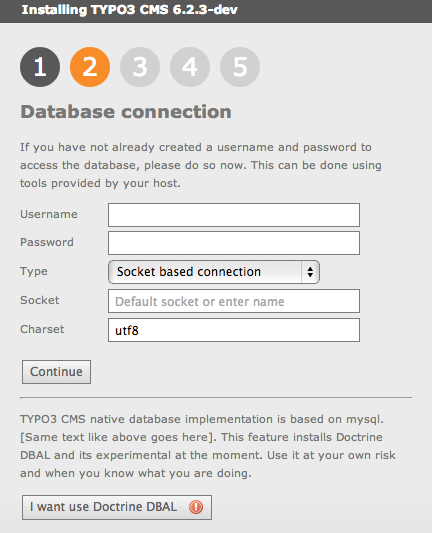
\includegraphics[width=\textwidth]{InstallingTYPO3/DoctrineDBAL/02-DatabaseConnection.png}
			\caption{Installation TYPO3 CMS mit Prototyp - Schritt 2a}
			\label{fig:installTYPO3DoctrineStepTwoA}
		\end{subfigure}%
		~ %add desired spacing between images, e. g. ~, \quad, \qquad, \hfill etc.
	%(or a blank line to force the subfigure onto a new line)
		\begin{subfigure}[b]{0.5\textwidth}
			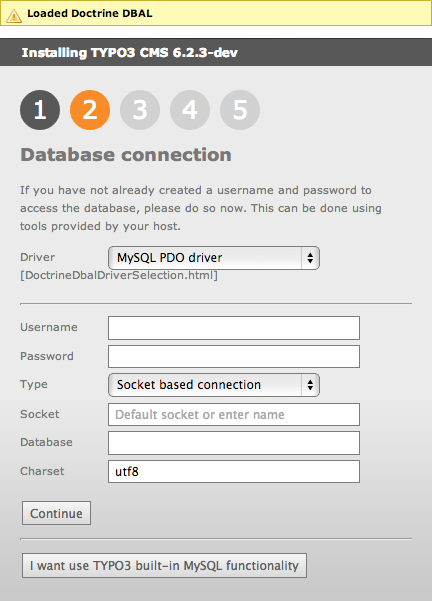
\includegraphics[width=\textwidth]{InstallingTYPO3/DoctrineDBAL/03-DatabaseConnectionDoctrineLoaded.png}
			\caption{Installation TYPO3 CMS mit Prototyp - Schritt 2b}
			\label{fig:installTYPO3DoctrineStepTwoB}
		\end{subfigure}
		~ %add desired spacing between images, e. g. ~, \quad, \qquad, \hfill etc.
	%(or a blank line to force the subfigure onto a new line)
		\caption{Installation von TYPO3 CMS mit den Prototyp}
		\label{fig:installationOfTYPO3}
	\end{figure}



Zur Überprüfung ob TYPO3 CMS tatsächlich den Prototypen nutzt, wurde in der \gls{ide} ein Debug-Breakpoint in\\ \phpinline{Konafets\DoctrineDbal\Persistence\Legacy\DatabaseConnection} innerhalb der \phpinline{connectDB} gesetzt, an dem die \gls{ide} die Ausführung von TYPO3 CMS anhielt als er erreicht wurde.


